Tale descrizione deve contemplare almeno gli elementi riportati nelle seguenti sottosezioni.

\subsection{Convolutional neural network}
\emph{Descrivere in questa sezione l’architettura della convolutional neural network
sviluppata nell’ambito del progetto. Se si utilizza un’architettura nota, si riportino gli elementi fondamentali della rete e le eventuali modifiche effettuate ma, soprattutto, si motivi la scelta.
Definire in ogni caso se la rete è stata progettata come regressore (output:
numero reale da 0 a 100 che rappresenta l’età, da approssimare all’intero più
vicino) o come classificatore (output: una delle 101 classi da 0 a 100) e fornire dettagli e motivazioni sulla funzione di costo scelta.}

L'architettura scelta è MobileNetV3 Large \cite{mobilenetv3}. Le reti neurali convoluzionali (CNNs) MobileNet sono conosciute per essere progettate pensando all'applicazione su sistemi mobili e/o embedded, cercando un trade-off tra prestazioni e risorse computazionali richieste. Hanno introdotto tecniche che migliorano l'efficienza, come la \emph{depthwise separable convolution} (MobileNetV1), i \emph{linear bottleneck} e la \emph{inverted residual structure} (MobileNetV2), la \emph{squeeze and excitation} (ResNet) e le funzioni di attivazione \emph{swish}. MobileNetV3, nelle sue versioni Small e Large, è il risultato di una combinazione di questi blocchi, ottimizzata tramite \emph{platform-aware NAS} e l'algoritmo \emph{NetAdapt} \cite{mobilenetv3}. 

Per essere efficiente, MobileNetV3 presenta un numero ridotto di pesi da addestrare rispetto ad altre architetture della letteratura, e ciò l'ha resa un ottimo candidato per l'addestramento con le risorse limitate di Google Colab (VRAM e 12 ore di tempo macchina). A parità di tempo, ci è possibile addestrare la rete su più immagini, quindi è possibile utilizzare un dataset estremamente ricco di campioni che, secondo i risultati di \cite{miviaage}, garantisce ottime prestazioni anche a reti più leggere.

Il nostro modello è una versione personalizzata dell'implementazione di MobileNetV3 Large sul framework Keras\footnote{\url{https://keras.io/api/applications/}}. Il modello viene adattato per diventare un regressore sostituendo il layer di classificazione con un layer di dimensione unitaria con attivazione lineare (ReLU). Questo ci ha permesso di astrarci dalla rappresentazione dell'età, in modo da lasciarla definita nell'intervallo \([0, +\infty)\), e di utilizzare la ben nota in letteratura Mean Squared Error (MSE) loss function
\begin{displaymath}
\text{MSE} = \frac{1}{n} \sum_{i=1}^{n} \left(Y_i - \hat{Y}_i\right),
\end{displaymath}
che tiene conto anche dell'entità della differenza tra la stima dell'età e la \emph{ground truth}.

\subsection{Procedura di addestramento}
\subsubsection{Dataset}
\label{subsubsec:dataset}

Il dataset utilizzato per addestrare la nostra rete a compiere il task assegnato è il dataset chiamato \emph{VGG-Face2 Mivia Age}, anche detto \emph{VMAGE}\cite{miviaage}.

Quest'ultimo dataset contiene $3.31$ milioni di immagini di 9131 soggetti. Ad ogni immagine è associata l'età del soggetto, tale valore è una stima dell'età apparente del soggetto catturato.
Il dataset ci è stato fornito già diviso in training set, che include $8631$ identità, e test set, che include le rimanenti 500.

\todo{Non mi piace la seguente frase, aiuto} Le risorse che \textit{Google Colab} mette a disposizione sono risultate insufficienti per allenare la rete sull'intero training set. È risultato necessario ridurre la grandezza di quest'ultimo, a tale scopo è stata svolta un analisi del training set e sono stati scelte le identità su cui svolgere l'addestramento della rete. Tale analisi è stata svolta anche con il supporto delle annotazioni per VGGFace2\footnote{Le annotazioni sono reperibili: \url{https://github.com/MiviaLab/GenderRecognitionFramework/releases/tag/0}}.

Con lo scopo di svolgere l'allenamento su un training set più bilanciato possibile, abbiamo svolto una prima analisi sul genere delle identità presenti.

\begin{figure}[H]

\begin{subfigure}{0.5\textwidth}
\def\svgscale{0.5}
\input{./Images/gender_ids.pdf_tex}
\caption{Identità divise per genere}
\label{sfig:Ids per gender}
\end{subfigure}
\begin{subfigure}{0.5\textwidth}
\def\svgscale{0.5}
\input{./Images/gender_images.pdf_tex}
\caption{Immagini divise per genere}
\label{sfig:Images per gender}
\end{subfigure}
\caption{Divisione per genere di identità e immagini}
\label{fig:gender_division}
\end{figure}

Come possiamo vedere in \ref{sfig:Ids per gender} e in \ref{sfig:Images per gender}, il training set risulta sbilanciato per quanto riguarda il genere dei soggetti.

L'analisi si è successivamente concentrata sulla \emph{media e deviazione standard} dell'età di ogni soggetto presente nel training set.

\begin{figure}[H]

\begin{subfigure}{0.5\textwidth}
\def\svgscale{0.42}
\input{./Images/n_ids_by_age_and_gender.pdf_tex}
\caption{Identità divise per genere ed età media}
\label{sfig:Ids per gender and mean age}
\end{subfigure}
\begin{subfigure}{0.5\textwidth}
\def\svgscale{0.42}
\input{./Images/n_images_by_age_and_gender.pdf_tex}
\caption{Immagini divise per genere ed età media}
\label{sfig:Images per gender and mean age}
\end{subfigure}
\caption{Divisione per genere di identità e immagini}
\label{fig:gender_age_division}
\end{figure}

Come si evince dai grafici in figura~\ref{sfig:Ids per gender and mean age} e in figura~\ref{sfig:Images per gender and mean age}, ci sono delle fasce d'età sovrarappresentate rispetto alle altre, in particolare le fasce d'età $[25,34]$ e $[35,44]$.

Con lo scopo di avere un training set quanto più bilanciato possibile, abbiamo scelto di escludere dal set gli uomini nelle fasce: $[25,34]$ e $[35,44]$; e le donne nella fascia $[25,34]$; la cui deviazione standard dell'età risulta inferiore a $5.5$. Il risultato di tale operazione è visibile in figura~\ref{fig:Ids per gender and mean age after the drop}.

\begin{figure}[H]
\centering
\def\svgscale{0.7}
\input{./Images/n_ids_by_age_and_gender_after_drop.pdf_tex}
\caption{Identità divise per genere ed età media dopo il taglio}
\label{fig:Ids per gender and mean age after the drop}
\end{figure}

Successivamente a tale operazione, al training set sono state sottratte ulteriori $500$ identità, scelte casualmente, che hanno formato il \emph{validation set}.

\subsubsection{Face detection}
\label{subsubsec:face_detection}

\emph{Descrivere il metodo utilizzato per effettuare il rilevamento del volto. Se si utilizza un approccio noto o i volti già estratti con framework esistenti, si specifichi questa informazione.}

Non è stato effettuato alcun rilevamento del volto. Nelle annotazioni del dataset VGGFAce2, già citate nella sezione~\ref{subsubsec:dataset}, sono riportate sia per il training set che per il test set, informazioni inerenti alle bounding boxes relative ai volti dei soggetti catturati. Tali informazioni definiscono quindi la \textbf{region of interest} (ROI) di ogni immagine.

\subsubsection{Face pre-processing} 

\emph{Descrivere e motivare tutte le tecniche di pre-processing applicate sulle immagini del volto.}

Si distinguono due fasi del pre-processing delle immagini, la prima fase viene effettuata a monte della data augmentation mentre la seconda a valle di quest'ultima.
Durante la prima fase viene ritagliato il volto del soggetto. Il ritaglio non viene effettuato però sulla ROI(sezione~\ref{subsubsec:face_detection}), infatti la region of interest viene allargata di un fattore $0.3$, ovviamente non andando oltre i limiti dettati dalla risoluzione dell'immagine. Tale operazione permette di ritagliare oltre al volto del soggetto l'intera testa.
Nella seconda fase ogni immagine viene ridimensionata alla risoluzione $224 \times 224$, nel caso in cui l'immagine dovesse essere ingrandita verrà utilizzata un interpolazione cubica, nel caso in cui, invece, l'immagine dovesse essere rimpicciolita verrà utilizzata un interpolazione area-based. Nonostante l'interpolazione cubica risulti più complessa e lenta dell'interpolazione lineare, è stata preferita a quest'ultima perché la qualità dell'immagine risultante sarà più alta. Il ridimensionamento viene effettuato mantenendo le proporzioni originali dell'immagine, nel caso in cui l'immagine non fosse quadrata vengono aggiunte delle bande nere che la rendono tale. Successivamente il valore medio di ogni canale è sottratto da ogni pixel\todo{specificare che la media è di VGGFace2}.

\begin{figure}[H]
\centering
\begin{subfigure}{0.3\textwidth}
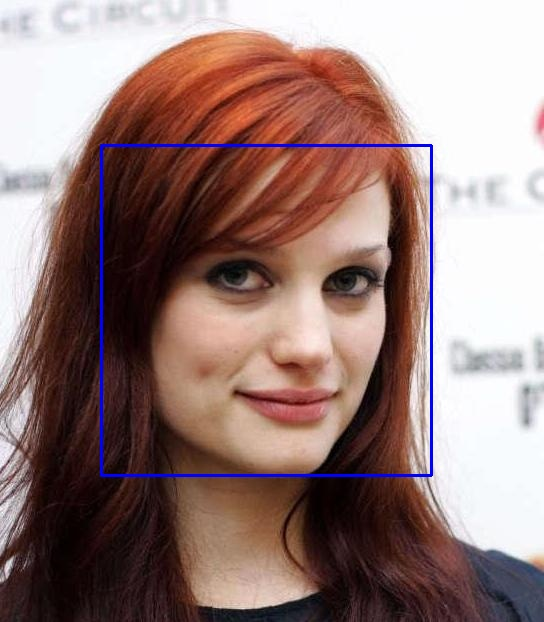
\includegraphics[width=\textwidth]{./Images/detection.jpg}
\caption{ROI evidenziata per quest'immagine}
\label{sfig:detection}
\end{subfigure}
\hspace{0.1\textwidth}
\begin{subfigure}{0.3\textwidth}
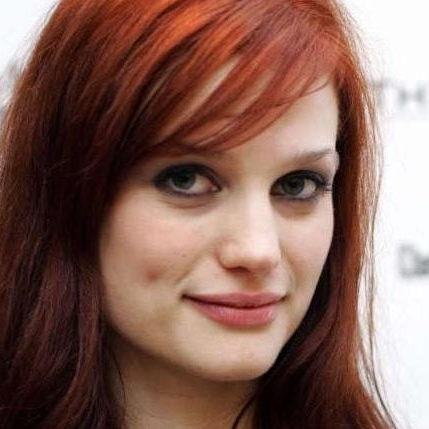
\includegraphics[width=\textwidth]{./Images/preprocessed.jpg}
\caption{Il risultato del ritaglio}
\label{sfig:preprocessed}
\end{subfigure}
\caption{Preprocessing a monte della data augmentation}
\label{fig:preprocessing}
\end{figure}

\subsubsection{Data augmentation}
\emph{Descrivere e motivare tutte le policy di augmentation implementate per estendere il dataset o per aumentarne la rappresentatività.}
Per la data augmentation, durante l'addestramento applichiamo una serie di filtri in maniera casuale. Lo scopo è quello di aumentare la rappresentatività del training set, con effetti riscontrabili nel tipo di immagini presenti in tutto il dataset, oltre che a fornire resilienza ad attacchi basilari.

I filtri applicati sono:
\begin{enumerate*}[label={\alph*)}]
\item \emph{rumore gaussiano additivo} con media 0 e deviazione standard nell'intervallo $[0.08, 0.30]$, come prevenzione ad attacchi semplici che sfruttano questo effetto;
\item \emph{blur gaussiano} con deviazione standard nell'intervallo $[1, 4]$, presente soprattutto in immagini di cui si fa un upscale tramite filtro bicubico;
\item \emph{ritaglio} \cite{miviagender}, per cui l'immagine viene tagliata ulteriormente per simulare facce coperte o fotografie in cui la faccia non è ripresa completamente;
\item \emph{rotazione} nell'intervallo $[-10 \degree, 10 \degree ]$, per rendere la rete invariante rispetto a facce non perfettamente allineate al frame;
\item \emph{rovesciamento} rispetto all'asse verticale;
\item \emph{inclinazione} \cite{miviagender} nello spazio tridimensionale;
\item \emph{spatter} \cite{miviagender}, ossia schizzi e macchie per rendere la rete invariante a possibili coperture del viso, sia digitali che volontarie da parte del soggetto inquadrato;
\item \emph{luminosità} nell'intervallo $[-50\%, 50\%]$ e \item \emph{contrasto} nell'intervallo $[0.1, 0.4] \cup [1.5, 5.0]$, per l'invarianza rispetto a condizioni di luce diverse.
\end{enumerate*}
Per ogni immagine, viene scelto casualmente se applicare o meno un filtro. In caso positivo, viene scelto casualmente uno dei filtri insieme ad un valore che ricada nell'intervallo predisposto per ognuno di essi. 

Gli intervalli sono stati scelti sulla base delle implementazioni del Mivia Gender Recognition Framework \cite{miviagender}, eventualmente personalizzati sulla base di alcune prove effettuate manualmente, tali per cui l'effetto non sia completamente distruttivo e il risultato sia ancora riconoscibile all'occhio umano rispetto all'immagine originale.

\begin{figure}[h]
\begin{subfigure}{0.2\textwidth}
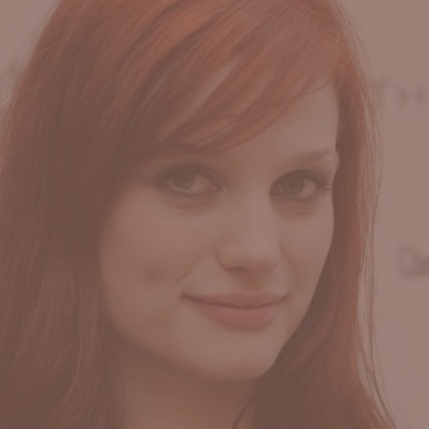
\includegraphics[width=\textwidth]{./Images/contrast_severity_0.2.jpg}
\caption{Contrasto aumentato di $0.2$}
\label{sfig:corruption_contrast}
\end{subfigure}\hfill
\begin{subfigure}{0.2\textwidth}
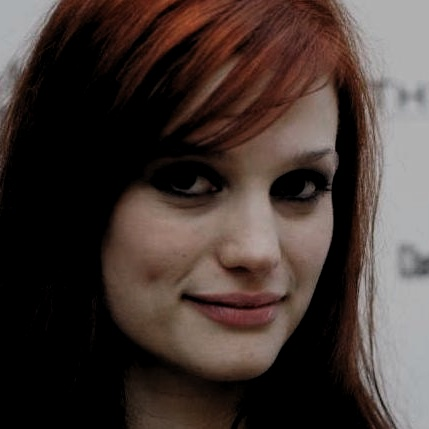
\includegraphics[width=\textwidth]{./Images/brightness_severity_-0.3.jpg}
\caption{Luminosità ridotta del $30\%$}
\label{sfig:corruption_brightness}
\end{subfigure}\hfill
\begin{subfigure}{0.2\textwidth}
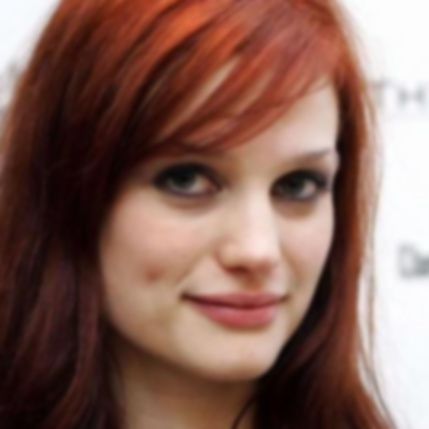
\includegraphics[width=\textwidth]{./Images/gaussian_blur_severity_2.0.jpg}
\caption{Blur gaussiana con deviazione standard $0.2$}
\label{sfig:corruption_gaussian_blur}
\end{subfigure}\hfill
\begin{subfigure}{0.2\textwidth}
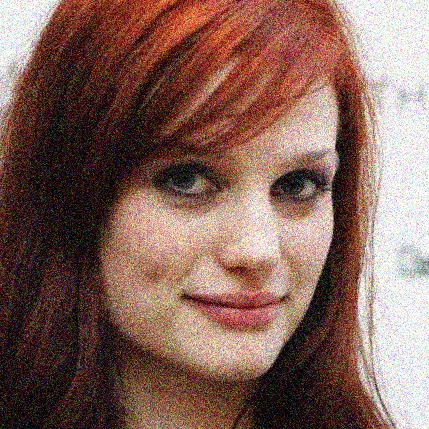
\includegraphics[width=\textwidth]{./Images/gaussian_noise_severity_0.1.jpg}
\caption{Rumore gaussiano con deviazione standard $0.1$}
\label{sfig:corruption_gaussian_noise}
\end{subfigure}\hfill

\begin{subfigure}{0.2\textwidth}
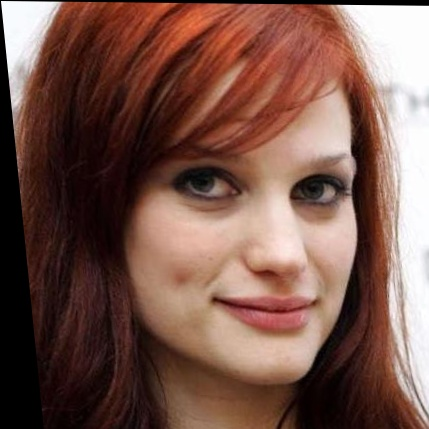
\includegraphics[width=\textwidth]{./Images/skew.jpg}
\caption{inclinazione nello spazio tridimensionale}
\label{sfig:corruption_skew}
\end{subfigure}\hfill
\begin{subfigure}{0.2\textwidth}
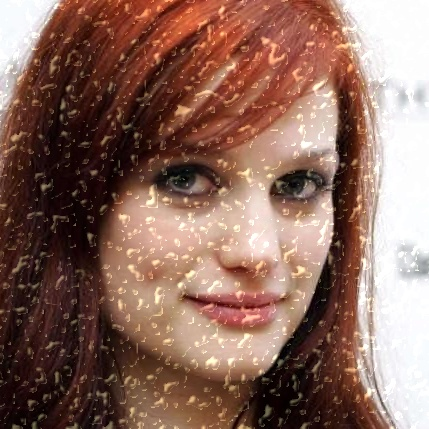
\includegraphics[width=\textwidth]{./Images/spatter_severity_3.jpg}
\caption{Spatter con severità $3.0$}
\label{sfig:corruption_spatter}
\end{subfigure}\hfill
\begin{subfigure}{0.2\textwidth}
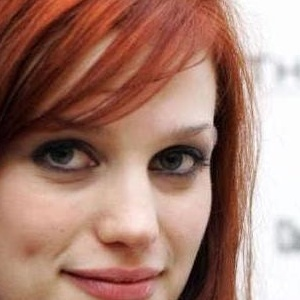
\includegraphics[width=\textwidth]{./Images/random_crop_severity_0.3.jpg}
\caption{Ritaglio del $30\%$}
\label{sfig:corruption_random_crop}
\end{subfigure}\hfill
\begin{subfigure}{0.2\textwidth}
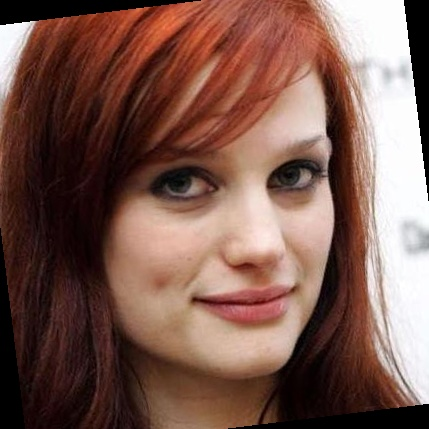
\includegraphics[width=\textwidth]{./Images/rotation_severity_7.0.jpg}
\caption{Rotazione di $7.0 \degree$}
\label{sfig:corruption_rotation}
\end{subfigure}\hfill
\caption{Possibili applicazioni dei filtri}
\label{sfig:data_augmentation}
\end{figure}

\subsubsection{Training from scratch o fine tuning}
\emph{Specificare se la rete viene addestrata con inizializzazione random o partendo da pesi pre-addestrati, motivando la scelta e fornendo dettagli sulla strategia di inizializzazione.}

\subsubsection{Procedura di training}
{\em Dettagliare e motivare almeno le seguenti scelte: numero di epoche di addestramento, tipo di ottimizzatore, learning rate scheduling (tecnica di riduzione, learning rate iniziale, fattore di riduzione). Fornire dettagli su eventuali elementi aggiuntivi: batch normalization, weight decay, early stopping etc. Per ognuna delle scelte, riportare i valori esatti dei parametri utilizzati, per rendere l’esperimento riproducibile. Motivare la scelta di tali valori.}